% ==============================================================================
% 第 9 章：基于自引用数据定义进行设计 (Chapter 9: Designing with Self-Referential Data Definitions)
% ==============================================================================

\chapter{基于自引用数据定义进行设计}
\label{sec:ch09_designing_lists}

初看之下，自引用数据定义似乎比之前的混合数据定义复杂得多。但正如上一章 \code{contains-flatt?} 的例子所展示的那样，程序设计配方的六个基本步骤依然完全适用。在本章中，我们将推广并细化设计配方，使其能够更加自然流畅地应对自引用数据定义。新内容主要涉及三个方面：识别何时需要自引用数据定义、推导函数模板、以及编写函数体。

\begin{recipebox}{处理任意大小数据的设计配方}
\begin{enumerate}
  \item \textbf{数据定义}：如果问题陈述涉及\textbf{任意大小}的信息，就必须使用自引用数据定义来表示它。目前为止你只见过一种此类定义——\code{List-of-names}。图~\ref{fig:arrows_for_self_references} 左侧展示了以同样方式定义的 \code{List-of-strings}。其他原子数据的列表定义也遵循完全相同的规律。
  
  一个有效的自引用数据定义必须满足两个先决条件：
  \begin{itemize}
    \item 必须包含至少两个分支（clause）；
    \item 至少有一个分支\textbf{不能}引用正在定义的数据类别本身（即\term{基本情况/基准条件}，base case）。
  \end{itemize}
  良好的编程习惯是用箭头明确标出自引用关系：从数据定义内部的引用指回被定义术语本身（如图~\ref{fig:arrows_for_self_references} 所示）。

  你必须通过构造数据示例来检验自引用定义的有效性。先从不含自引用的分支开始生成第一个示例；接着使用包含自引用的分支，将前面生成的示例代入自引用位置以生成更大的示例：
\begin{lstlisting}[language=BSL]
'()
(cons "a" '())
(cons "b" (cons "a" '()))
\end{lstlisting}
  如果无法从数据定义生成示例，则该定义是无效的；如果你能生成示例但无法构造出规模递增的示例，则该定义可能无法契合其预期解释。

  \item \textbf{函数签名、目的说明与函数头}：函数头部材料与以往毫无二致：签名、目的说明和桩定义。在构思目的说明时，\textbf{务必关注函数计算什么，而非如何计算}，尤其不要过早考虑如何遍历给定的数据。例如：
\begin{lstlisting}[language=BSL]
; List-of-strings -> Number
; 计算 alos 中包含多少个字符串
(define (how-many alos)
  0)
\end{lstlisting}
  目的说明清晰指明了函数只负责统计字符串个数，无需预先设想如何在 BSL 中实现它。

  \item \textbf{功能示例}：在构思功能示例时，务必多次运用数据定义中的自引用分支来构造测试输入。这是后续确保测试用例覆盖整个函数定义的最佳途径：
\begin{lstlisting}[language=BSL]
(check-expect (how-many '()) 0)
(check-expect (how-many (cons "a" '())) 1)
(check-expect (how-many (cons "b" (cons "a" '()))) 2)
\end{lstlisting}

  \item \textbf{模板}：自引用数据定义本质上仍是分类数据定义，因此模板开发遵循第 6 章的规则。\code{cond} 表达式的分支数与数据定义的分支数完全一致；每个分支的条件对应数据定义的识别条件；在处理复合值的每个分支中写下相应的选择器表达式。
  
  图~\ref{fig:translate_data_def_to_template} 以问答形式阐明了这一过程。如果对消耗 \code{List-of-strings} 的函数应用这些规则，初步得到以下形态：
\begin{lstlisting}[language=BSL]
(define (fun-for-los alos)
  (cond
    [(empty? alos) ...]
    [(cons? alos)
     (... (first alos) ... (rest alos) ...)]))
\end{lstlisting}
  请牢记，模板的目的是将数据定义的结构转化为函数代码的骨架。当数据定义在第 $i$ 个分支的第 $k$ 个字段存在自引用时，模板就必须在第 $i$ 个分支对第 $k$ 个字段的选择器调用上建立\textbf{递归调用}！
  
  在文本代码中，我们通过函数的自调用（self-application）来代替箭头：
\begin{lstlisting}[language=BSL]
(define (fun-for-los alos)
  (cond
    [(empty? alos) ...]
    [(cons? alos)
     (... (first alos) ...
      ... (fun-for-los (rest alos)) ...)]))
\end{lstlisting}
  我们将函数的自我调用称为\term{递归}（recursion），在本书前四部分特称为\term{自然递归}（natural recursion）。

  \item \textbf{函数体编写}：从不含递归调用的分支（基本情况）开始编写，其答案通常显而易见或已在示例中给出。
  
  接着处理自引用分支。牢记模板中每个表达式计算的是什么。对于自然递归 \code{(fun-for-los (rest alos))}，\textbf{假定该函数已经按照目的说明正确工作}。这虽然看似是一次“信念之跃”（leap of faith），但它在数学归纳法（Induction Theorem）的保证下永远有效！剩下的工作只是将提取的值与递归调用的结果组合起来。

  \item \textbf{测试}：将所有示例转化为测试用例，确保全部通过，并检查测试覆盖了函数的所有分支。
\end{enumerate}
\end{recipebox}

\begin{figure}[htbp]
  \centering
  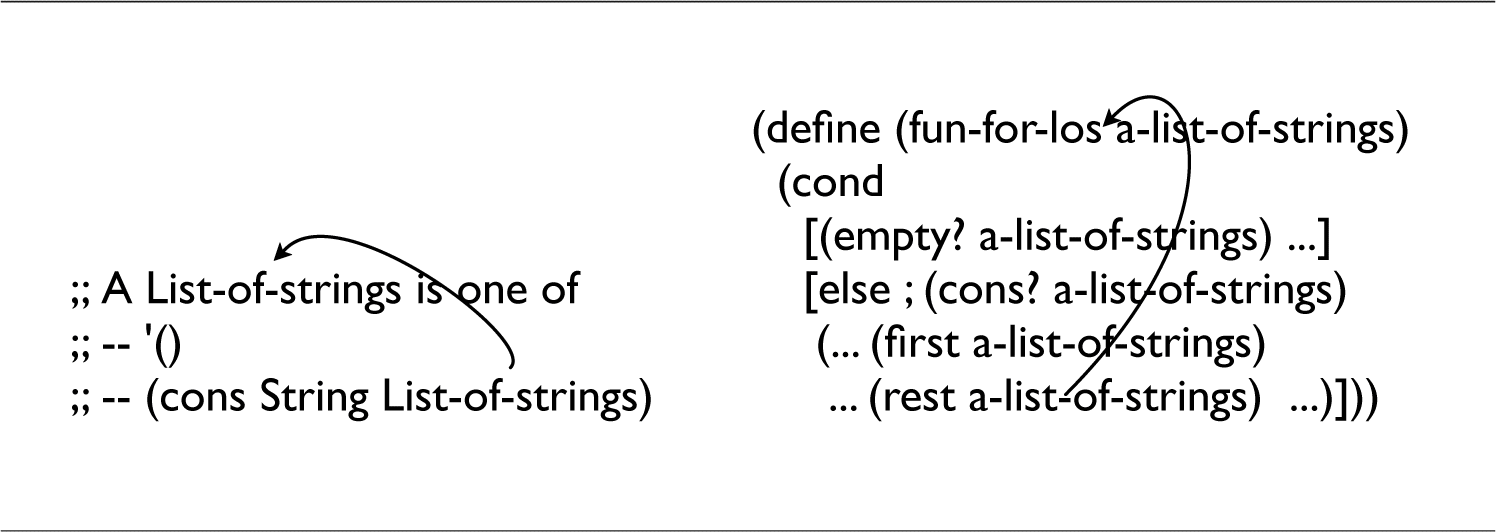
\includegraphics[width=0.85\textwidth]{images/00182.png}
  \caption{数据定义与模板中的自引用箭头映射}
  \label{fig:arrows_for_self_references}
\end{figure}

\begin{figure}[htbp]
  \centering
  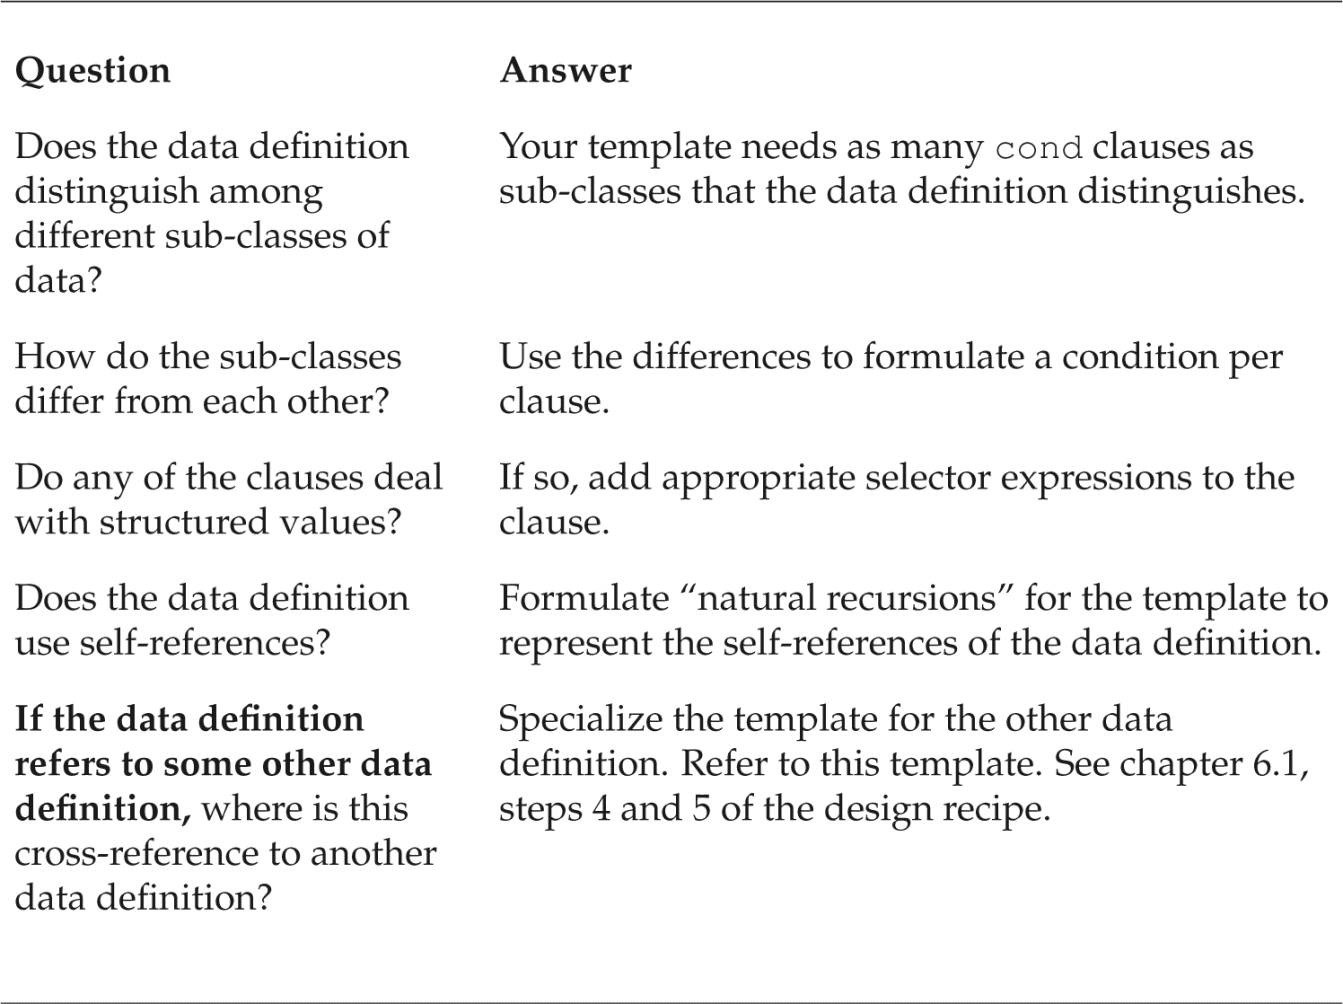
\includegraphics[width=0.85\textwidth]{images/00185.png}
  \caption{如何将数据定义转换为模板}
  \label{fig:translate_data_def_to_template}
\end{figure}

\begin{figure}[htbp]
  \centering
  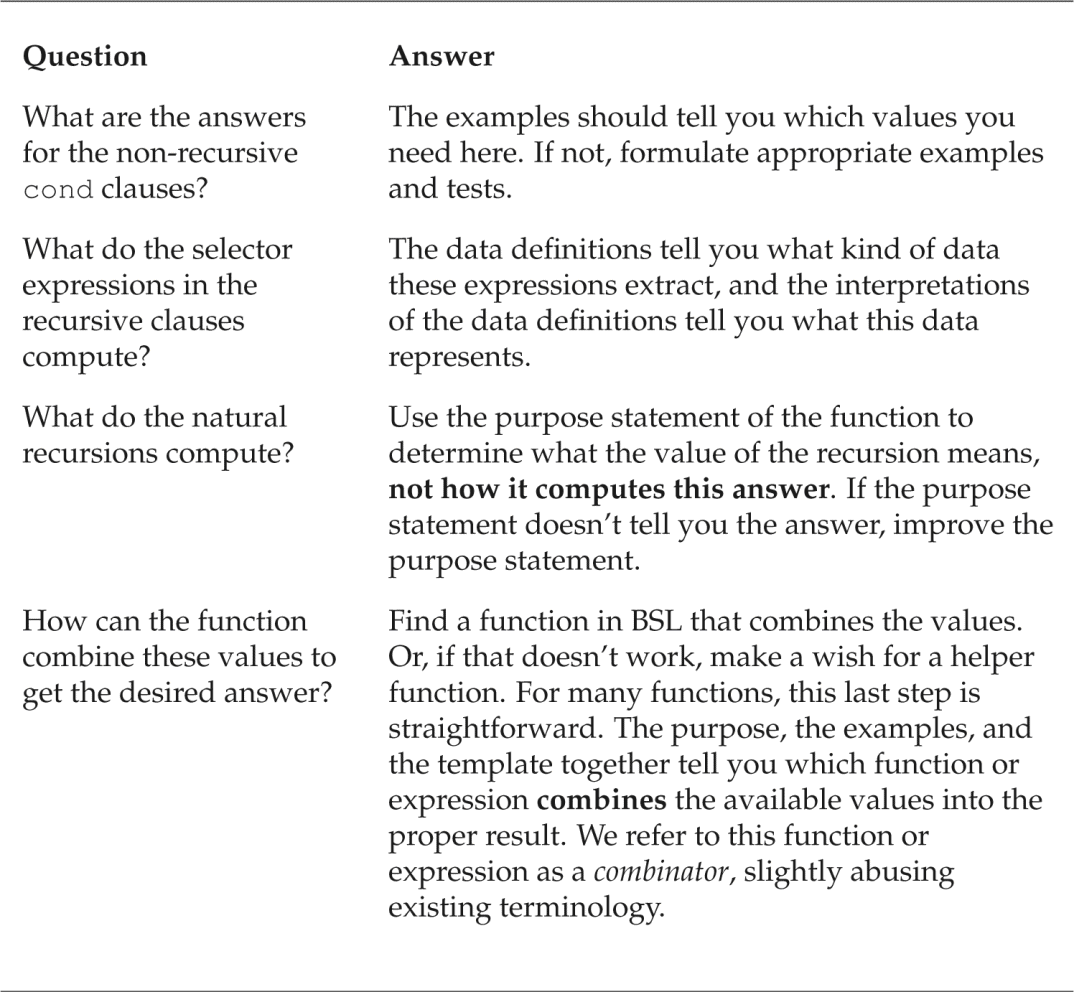
\includegraphics[width=0.85\textwidth]{images/00189.png}
  \caption{如何将模板转换为函数定义}
  \label{fig:turn_template_into_function}
\end{figure}

对于 \code{how-many}，基本情况为 \code{'()}，结果显然是 \code{0}。在第二分支中，\code{(first alos)} 得到首个字符串，\code{(how-many (rest alos))} 算出剩余列表的字符串个数。为了求出整个列表的长度，只需将递归结果加 \code{1}：
\begin{lstlisting}[language=BSL]
(define (how-many alos)
  (cond
    [(empty? alos) 0]
    [else (+ (how-many (rest alos)) 1)]))
\end{lstlisting}

\begin{notebox}[表格辅助法]
初学者在寻找组合函数（用于将首项与剩余项递归结果结合起来的辅助操作）时有时会感到困难。此时可以借助\term{表格辅助法}（如图~\ref{fig:table_method} 和图~\ref{fig:tabulating_args} 所示）：列出输入样例、模板中各子表达式的值以及期望的最终结果。观察自然递归列与期望结果列的数值差异，往往能一眼猜出所需的组合操作！
\end{notebox}

\begin{figure}[htbp]
  \centering
  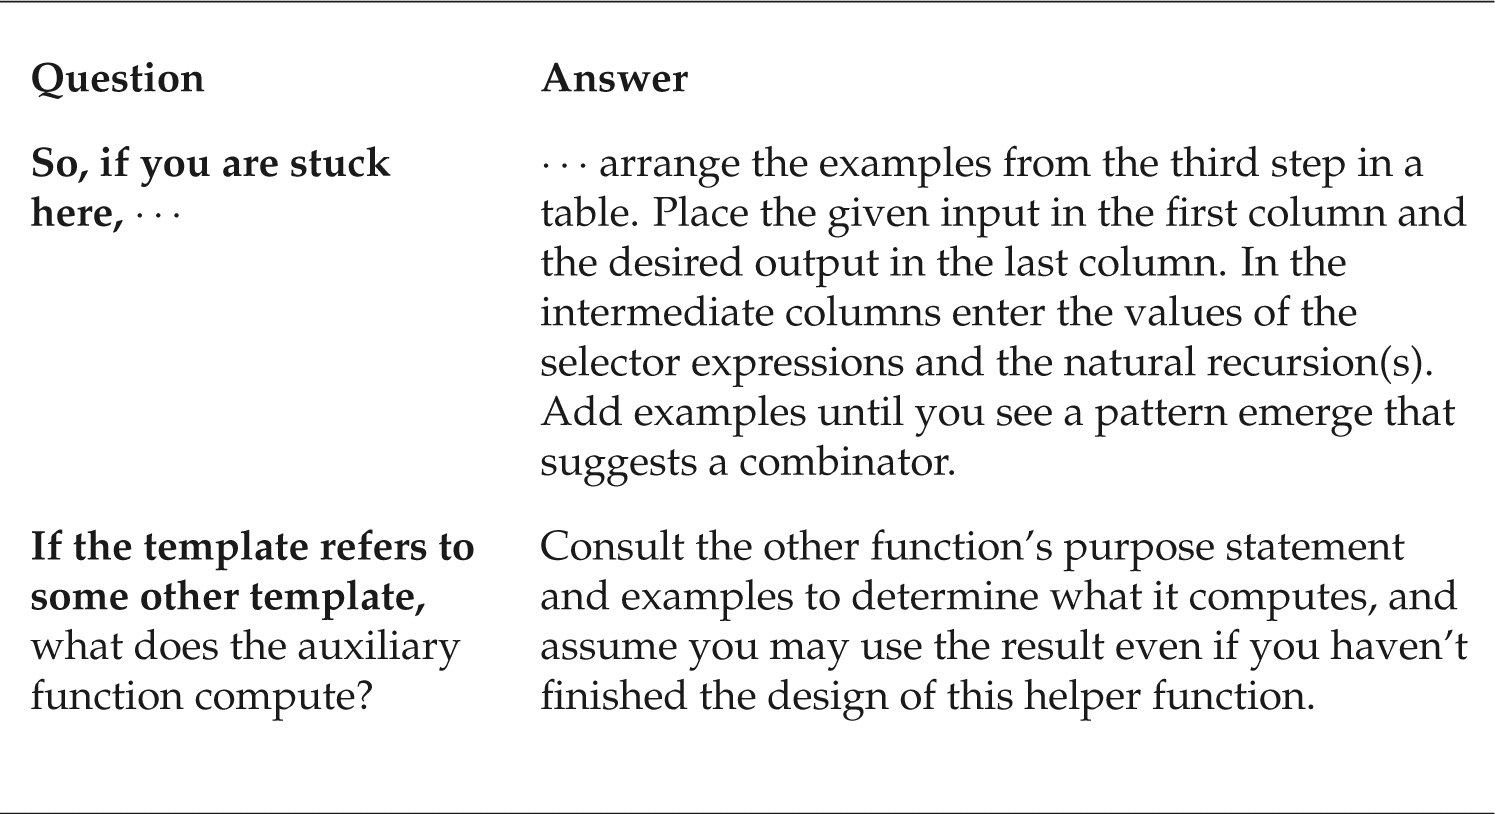
\includegraphics[width=0.8\textwidth]{images/00190.png}
  \caption{将模板转化为函数的表格方法}
  \label{fig:table_method}
\end{figure}

\begin{figure}[htbp]
  \centering
  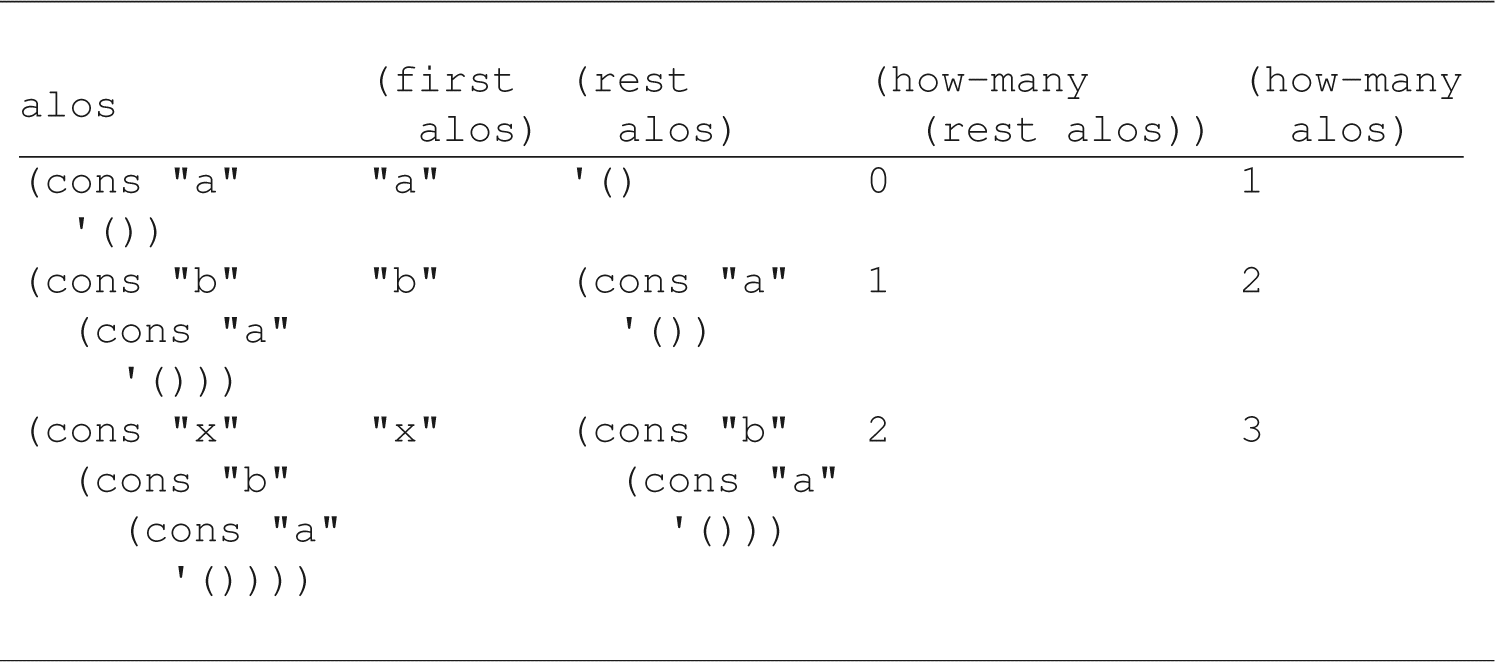
\includegraphics[width=0.8\textwidth]{images/00191.png}
  \caption{制表演算参数、中间值与结果}
  \label{fig:tabulating_args}
\end{figure}

图~\ref{fig:design_recipe_self_referential} 总结了针对自引用数据的完整设计配方表格。

\begin{figure}[htbp]
  \centering
  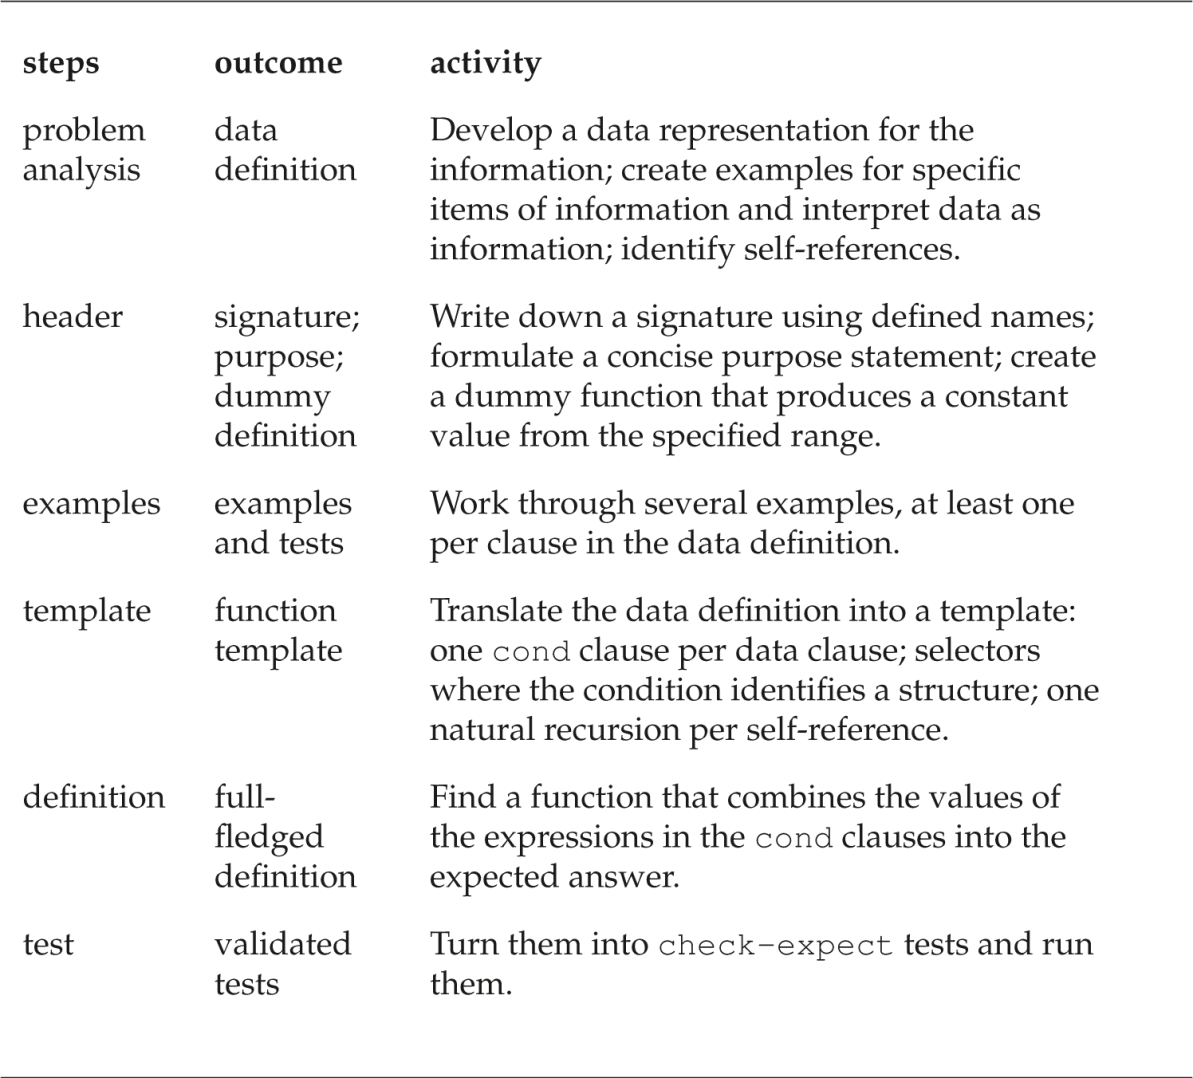
\includegraphics[width=0.9\textwidth]{images/00192.png}
  \caption{针对自引用数据设计函数的完整配方}
  \label{fig:design_recipe_self_referential}
\end{figure}

\section{练手习题：列表}
\label{sec:ch09_finger_exercises_lists}

\begin{exercise}{对比模板}{137}
比较 \code{contains-flatt?} 与 \code{how-many} 的模板。如果忽略函数名称，它们是完全相同的。请解释这种相似性的根源。
\end{exercise}

\begin{exercise}{金额求和函数 sum}{138}
以下是表示金额序列的数据定义：
\begin{lstlisting}[language=BSL]
; A List-of-amounts 是以下之一：
; -- '()
; -- (cons PositiveNumber List-of-amounts)
\end{lstlisting}
创建一些示例以确保你理解该数据定义，并在纸上画出标明自引用的箭头。

设计函数 \code{sum}，接收一个 \code{List-of-amounts} 并计算所有金额的总和。使用 DrRacket 的单步求值器观察 \code{(sum l)} 在短列表上的执行过程。
\end{exercise}

\begin{exercise}{数字列表验证与防御性求和}{139}
观察以下数据定义：
\begin{lstlisting}[language=BSL]
; A List-of-numbers 是以下之一：
; -- '()
; -- (cons Number List-of-numbers)
\end{lstlisting}
该类别的某些元素可以作为练习 138 中 \code{sum} 的合法输入，而另一些则不行。

设计函数 \code{pos?}，接收一个 \code{List-of-numbers} 并判断其中所有数字是否均为正数。换言之，若 \code{(pos? l)} 返回 \code{\#true}，则 \code{l} 同时也是 \code{List-of-amounts} 的元素。使用单步求值器观察 \code{pos?} 在 \code{(cons 5 '())} 和 \code{(cons -1 '())} 上的求值过程。

接着设计带校验的求和函数 \code{checked-sum}：接收一个 \code{List-of-numbers}。如果输入同时属于 \code{List-of-amounts}，则计算其总和；否则报错（提示：使用 \code{check-error} 进行测试）。

最后，思考如果直接对任意 \code{List-of-numbers} 应用练习 138 中的 \code{sum}，它会计算出什么？
\end{exercise}

\begin{exercise}{布尔值列表判定}{140}
设计函数 \code{all-true}，接收一个布尔值列表并判断其所有元素是否均为 \code{\#true}。也就是说，只要列表中存在任何 \code{\#false}，函数就返回 \code{\#false}。

接着设计函数 \code{one-true}，判断列表中是否至少有一个元素为 \code{\#true}。

在编写代码时尝试使用表格辅助法，它能帮你准确确定基本情况的返回值。使用单步求值器观察这些函数在 \code{(cons \#true '())}、\code{(cons \#false '())} 以及 \code{(cons \#true (cons \#false '()))} 上的运行轨迹。
\end{exercise}

\begin{exercise}{字符串拼接函数 cat}{141}
如果要设计函数 \code{cat}，接收一个字符串列表并将其拼接为一个长字符串，你必然会得到以下部分定义：
\begin{lstlisting}[language=BSL]
(define (cat los)
  (cond
    [(empty? los) ...]
    [else (... (first los) ... (cat (rest los)) ...)]))
\end{lstlisting}
完成图~\ref{fig:table_for_cat} 中的表格，猜出能够将子表达式的值组合为期望结果的函数。
使用单步求值器观察 \code{(cat (cons "a" '()))} 的求值。
\end{exercise}

\begin{figure}[htbp]
  \centering
  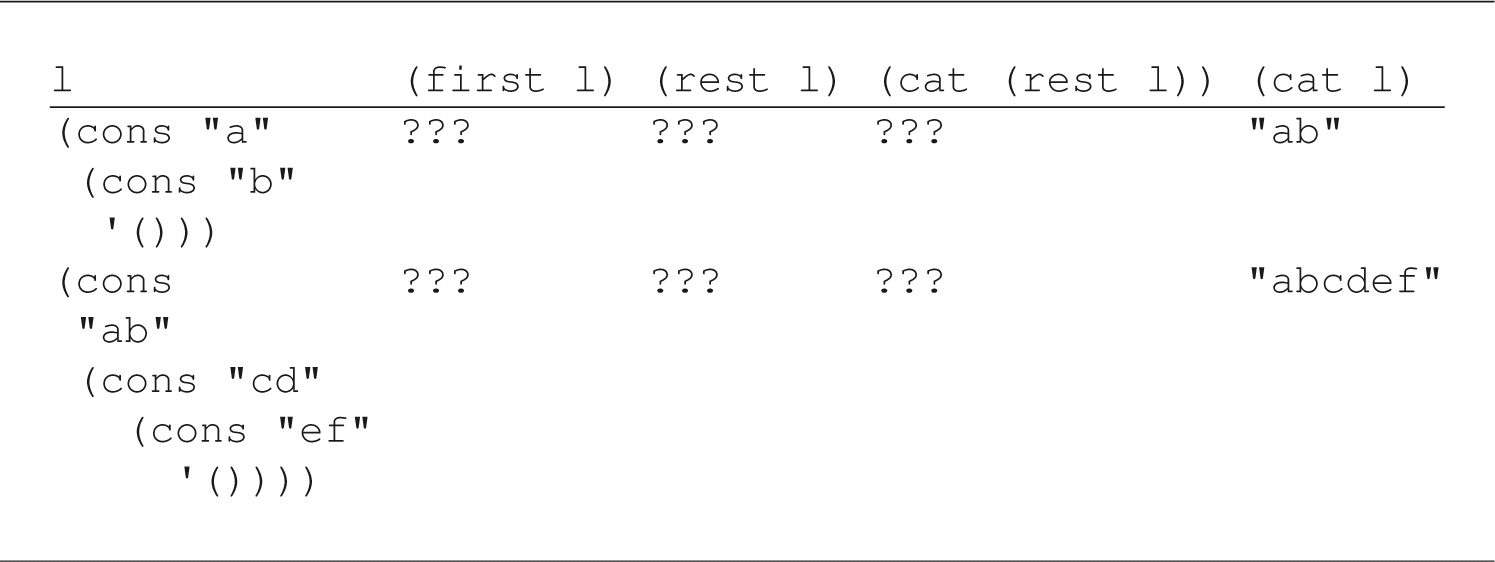
\includegraphics[width=0.8\textwidth]{images/00194.png}
  \caption{函数 cat 的辅助推导表}
  \label{fig:table_for_cat}
\end{figure}

\begin{exercise}{查找不合尺寸的图像 ill-sized?}{142}
设计函数 \code{ill-sized?}，消耗图像列表 \code{loi} 和一个正数 $n$。它返回 \code{loi} 中第一张\textbf{不是} $n \times n$ 正方形的图像；若所有图像均符合尺寸要求，则返回 \code{\#false}。

提示：在函数签名的结果部分使用以下数据定义：
\begin{lstlisting}[language=BSL]
; ImageOrFalse 是以下之一：
; -- Image
; -- #false
\end{lstlisting}
\end{exercise}

\section{非空列表}
\label{sec:ch09_non_empty_lists}

现在你已经掌握了使用 \code{cons} 以及构建列表数据定义的基础。本节我们将探讨一种在实践中极为常见的数据结构：\term{非空列表}（non-empty list）。

让我们从计算温度列表的平均值这一看似简单的问题开始：
\begin{lstlisting}[language=BSL]
; A List-of-temperatures 是以下之一：
; -- '()
; -- (cons CTemperature List-of-temperatures)

; A CTemperature 是大于 -272 的 Number。
\end{lstlisting}

直接按照之前的常规模板设计 \code{average} 函数：
\begin{lstlisting}[language=BSL]
(define (average alot)
  (cond
    [(empty? alot) ...]
    [(cons? alot)
     (... (first alot) ... (average (rest alot)) ...)]))
\end{lstlisting}
然而，要将这个模板转化为函数体却极为困难！首先，在 \code{empty?} 分支中需要返回空温度集的平均值，但在数学上并不存在这样的数字（除以零无定义）。其次，在第二分支中需要将一个新温度与剩余温度的平均值组合，这种增量式均值计算极不自然。

在小学算术中，计算平均值的方法是将所有温度相加，然后除以温度的个数。这个常识告诉我们：\code{average} 实际上由三个子任务构成：求和（summing）、计数（counting）和相除（dividing）。根据“单一函数负责单一任务”的设计准则，代码自然应当这样组织：
\begin{lstlisting}[language=BSL]
; List-of-temperatures -> Number
; 计算给定温度列表的平均值
(define (average alot)
  (/ (sum alot) (how-many alot)))

; List-of-temperatures -> Number
; 对列表中的所有温度求和
(define (sum alot)
  (cond
    [(empty? alot) 0]
    [else (+ (first alot) (sum (rest alot)))]))
\end{lstlisting}

然而，当输入为空列表 \code{'()} 时，\code{average} 会因为 \code{(/ 0 0)} 而发生除以零错误。

\begin{exercise}{带校验的平均值计算}{143}
在 DrRacket 中测试 \code{average} 应用于空列表时的表现。接着设计 \code{checked-average} 函数，当输入为 \code{'()} 时抛出具有说明性的错误信息。
\end{exercise}

另一种更根本的解决方案是在函数签名中明确排除空列表：
\begin{lstlisting}[language=BSL]
; An NEList-of-temperatures（非空温度列表）是以下之一：
; -- (cons CTemperature '())
; -- (cons CTemperature NEList-of-temperatures)
; 解释：非空的摄氏温度列表
\end{lstlisting}

请注意这一数据定义的精妙之处：它的两个分支都是 \code{cons} 结构，区别在于其 \code{rest} 字段：基准分支的 \code{rest} 恒为 \code{'()}，而自引用分支的 \code{rest} 是另一个非空列表！

因此，区分这两类的谓词应当是：提取 \code{rest} 字段并检查其是否为 \code{empty?}：
\begin{lstlisting}[language=BSL]
; NEList-of-temperatures -> Number
; 针对非空列表的函数模板
(define (sum ne-l)
  (cond
    [(empty? (rest ne-l)) (first ne-l)]
    [else (+ (first ne-l) (sum (rest ne-l)))]))
\end{lstlisting}

\begin{exercise}{sum 和 how-many 的兼容性}{144}
为 \code{List-of-temperatures} 设计的 \code{sum} 和 \code{how-many} 是否能直接应用于 \code{NEList-of-temperatures}？如果认为不行，请给出反例；如果认为可以，请说明理由。
\end{exercise}

\begin{exercise}{降序判断 sorted>?}{145}
设计谓词 \code{sorted>?}，接收一个 \code{NEList-of-temperatures}。如果温度按降序排列（即后一个温度严格小于前一个），则返回 \code{\#true}；否则返回 \code{\#false}。

提示：参考图~\ref{fig:table_for_sorted} 中的辅助表格，填补未完成的行，并推导出组合表达式。
\end{exercise}

\begin{figure}[htbp]
  \centering
  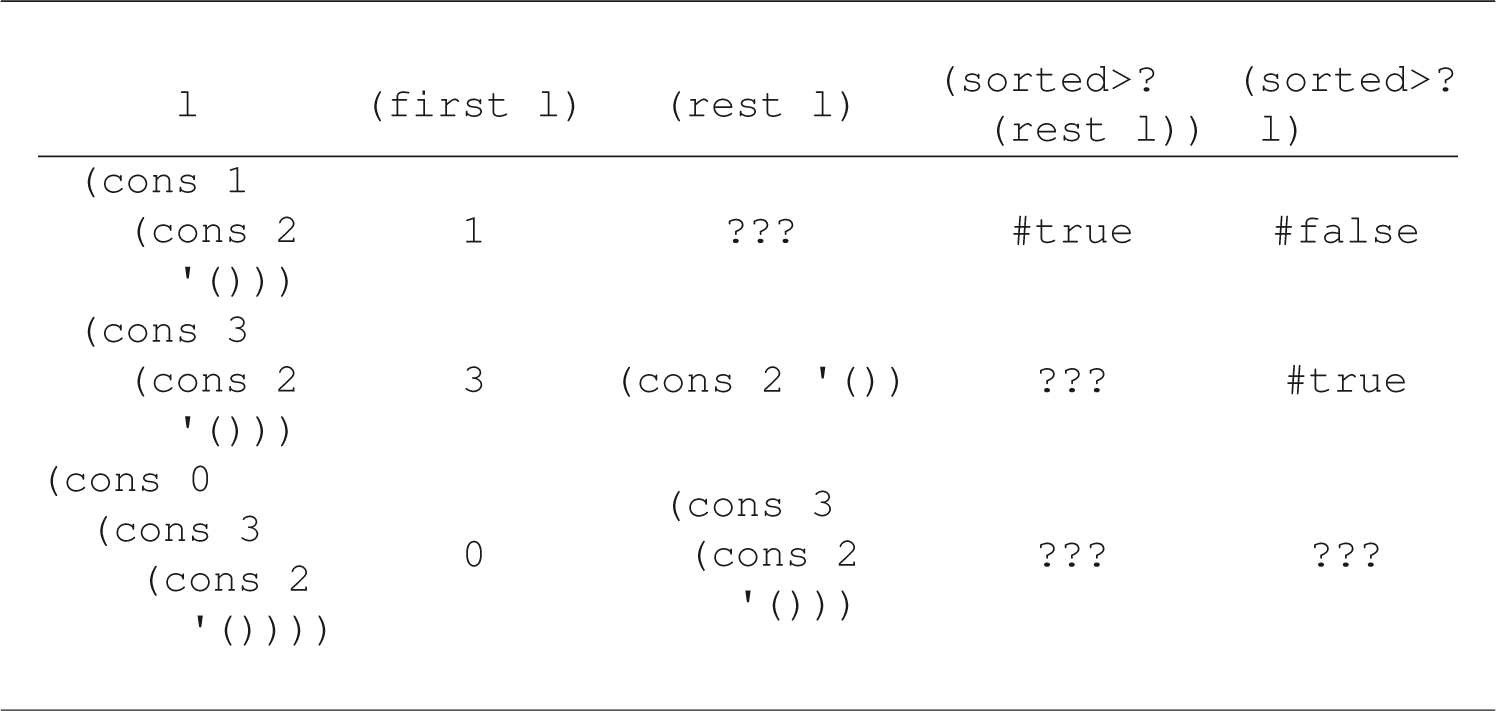
\includegraphics[width=0.8\textwidth]{images/00197.png}
  \caption{sorted>? 辅助推导表}
  \label{fig:table_for_sorted}
\end{figure}

\begin{exercise}{非空列表的 how-many}{146}
为 \code{NEList-of-temperatures} 设计专门的 \code{how-many} 函数，并确保以此重构的 \code{average} 通过所有测试。
\end{exercise}

\begin{exercise}{非空布尔列表}{147}
给出 \code{NEList-of-Booleans}（非空布尔值列表）的数据定义，并重新设计练习 140 中的 \code{all-true} 与 \code{one-true}。
\end{exercise}

\begin{exercise}{设计取舍探讨}{148}
比较本节中针对非空列表设计的函数与前一节支持空列表的函数。允许空列表的数据定义与强制非空的数据定义相比，在软件设计中孰优孰劣？为什么？
\end{exercise}

\section{自然数}
\label{sec:ch09_natural_numbers}

BSL 提供了诸如 \code{make-list} 的内置函数：它消耗一个数字 $n$ 和另一个值 $v$，产生一个包含 $n$ 个 $v$ 的列表：
\begin{replbox}
> (make-list 2 "hello")
(cons "hello" (cons "hello" '()))
> (make-list 3 #true)
(cons #true (cons #true (cons #true '())))
> (make-list 0 17)
'()
\end{replbox}

尽管它接受的是原子数据（数字），却能产生任意大小的数据！这是如何做到的？
答案在于：此处的数字并非一般的实数，而是特殊的\term{自然数}（Natural Numbers，用于计数的数）。自然数本身就是一个典型的自引用数据定义：
\begin{lstlisting}[language=BSL]
; An N（自然数）是以下之一：
; -- 0
; -- (add1 N)
; 解释：表示非负计数数字
\end{lstlisting}

第一分支表明 \code{0} 是一个自然数（表示没有被计数的对象）；第二分支表明若 $n$ 是自然数，则通过 \code{(add1 n)} 构造出的数也是自然数。在这里，\code{add1} 的角色宛如列表中的 \code{cons}，而它的配对函数 \code{sub1}（减 1）则相当于选择器！谓词 \code{zero?} 用于检查是否为基准值 \code{0}，而 \code{positive?} 用于检查是否大于 0。

基于这一自引用定义，我们来设计复制函数 \code{copier}：
\begin{lstlisting}[language=BSL]
; N String -> List-of-strings
; 创建由 n 个字符串 s 构成的列表
(check-expect (copier 0 "hello") '())
(check-expect (copier 2 "hello") (cons "hello" (cons "hello" '())))

(define (copier n s)
  (cond
    [(zero? n) '()]
    [(positive? n) (cons s (copier (sub1 n) s))]))
\end{lstlisting}

\begin{figure}[htbp]
  \centering
  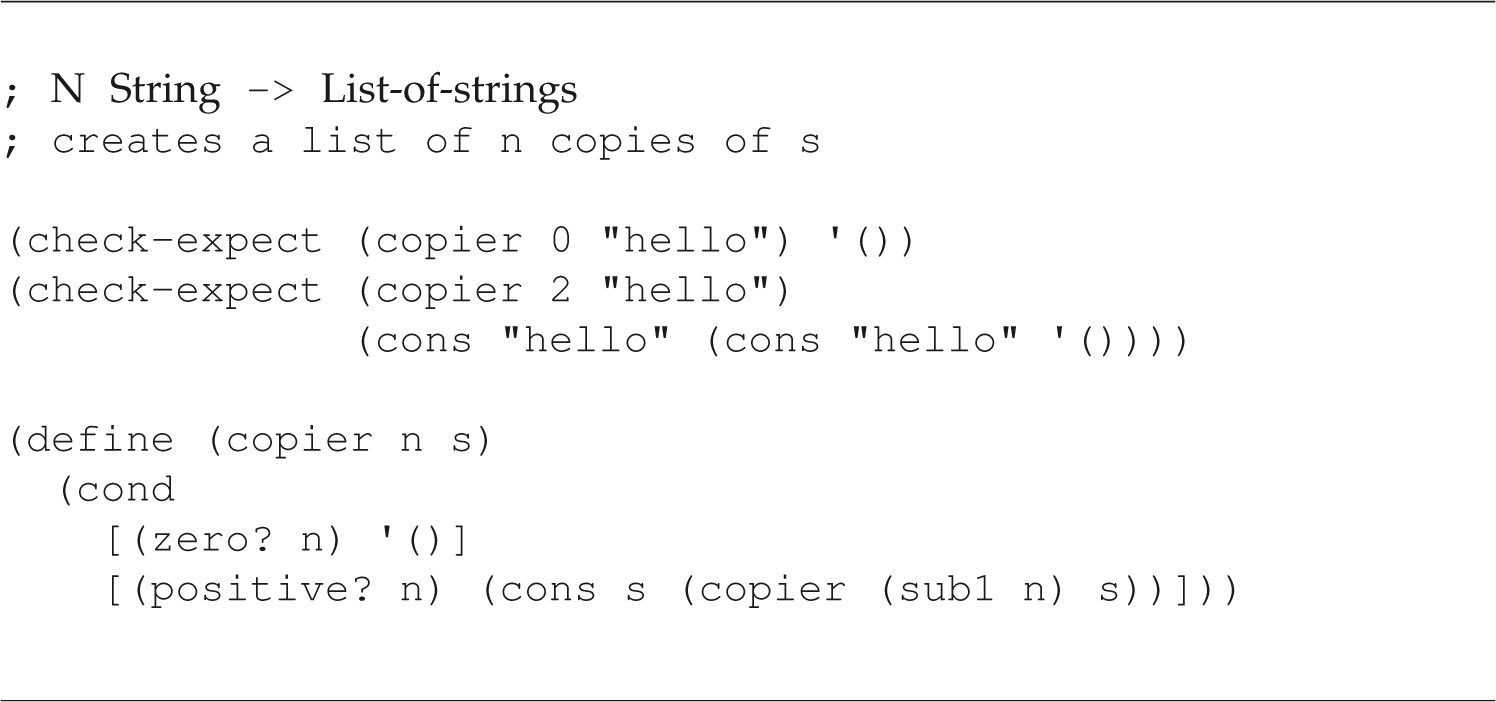
\includegraphics[width=0.85\textwidth]{images/00199.png}
  \caption{创建复制项列表}
  \label{fig:copier_definition}
\end{figure}

\begin{exercise}{类型通用性与条件分支}{149}
如果将 \code{copier} 应用于自然数和布尔值或图像，它能正常工作吗？

另外，考虑以下使用 \code{else} 的变体：
\begin{lstlisting}[language=BSL]
(define (copier.v2 n s)
  (cond
    [(zero? n) '()]
    [else (cons s (copier.v2 (sub1 n) s))]))
\end{lstlisting}
当分别对 \code{copier} 和 \code{copier.v2} 输入 \code{0.1} 和 \code{"x"} 时，二者的行为有何区别？请使用单步求值器加以验证。
\end{exercise}

\begin{exercise}{不用加号实现累加}{150}
设计函数 \code{add-to-pi}：消耗自然数 $n$，在\textbf{不使用}内置 \code{+} 运算符的前提下将其与 $\pi$ 相加。
\begin{lstlisting}[language=BSL]
; N -> Number
; 在不使用 + 的情况下计算 (+ n pi)
(check-within (add-to-pi 3) (+ 3 pi) 0.001)
(define (add-to-pi n)
  pi)
\end{lstlisting}
完成后，将其推广为通用函数 \code{add}：在不使用 \code{+} 的情况下将自然数 $n$ 与任意数 $x$ 相加。为什么测试桩代码中使用 \code{check-within}？
\end{exercise}

\begin{exercise}{不用乘号实现乘法}{151}
设计函数 \code{multiply}：消耗自然数 $n$ 与数字 $x$，在\textbf{不使用}内置 \code{*} 运算符的前提下计算两者的乘积。它与小学所学的乘法算理有何联系？
\end{exercise}

\begin{exercise}{排列图像：列与行}{152}
设计两个图像排列函数：
\begin{itemize}
  \item \code{col}：消耗自然数 $n$ 和图像 \code{img}，纵向垂直排列生成由 $n$ 个 \code{img} 组成的单列长图；
  \item \code{row}：消耗自然数 $n$ 和图像 \code{img}，横向水平排列生成由 $n$ 个 \code{img} 组成的单行长图。
\end{itemize}
\end{exercise}

\begin{exercise}{模拟教室气球袭击}{153}
利用练习 152 的函数生成一个 $8 \times 18$ 的网格矩形，每个小方格为 $10 \times 10$ 像素，放置在同等大小的空画板中作为阶梯教室。

设计函数 \code{add-balloons}：接收一个坐标落在教室范围内的 \code{Posn} 列表，产生带有红色圆点（模拟油漆水球着击点）的教室渲染图（如图~\ref{fig:random_attacks} 所示）。
\end{exercise}

\begin{figure}[htbp]
  \centering
  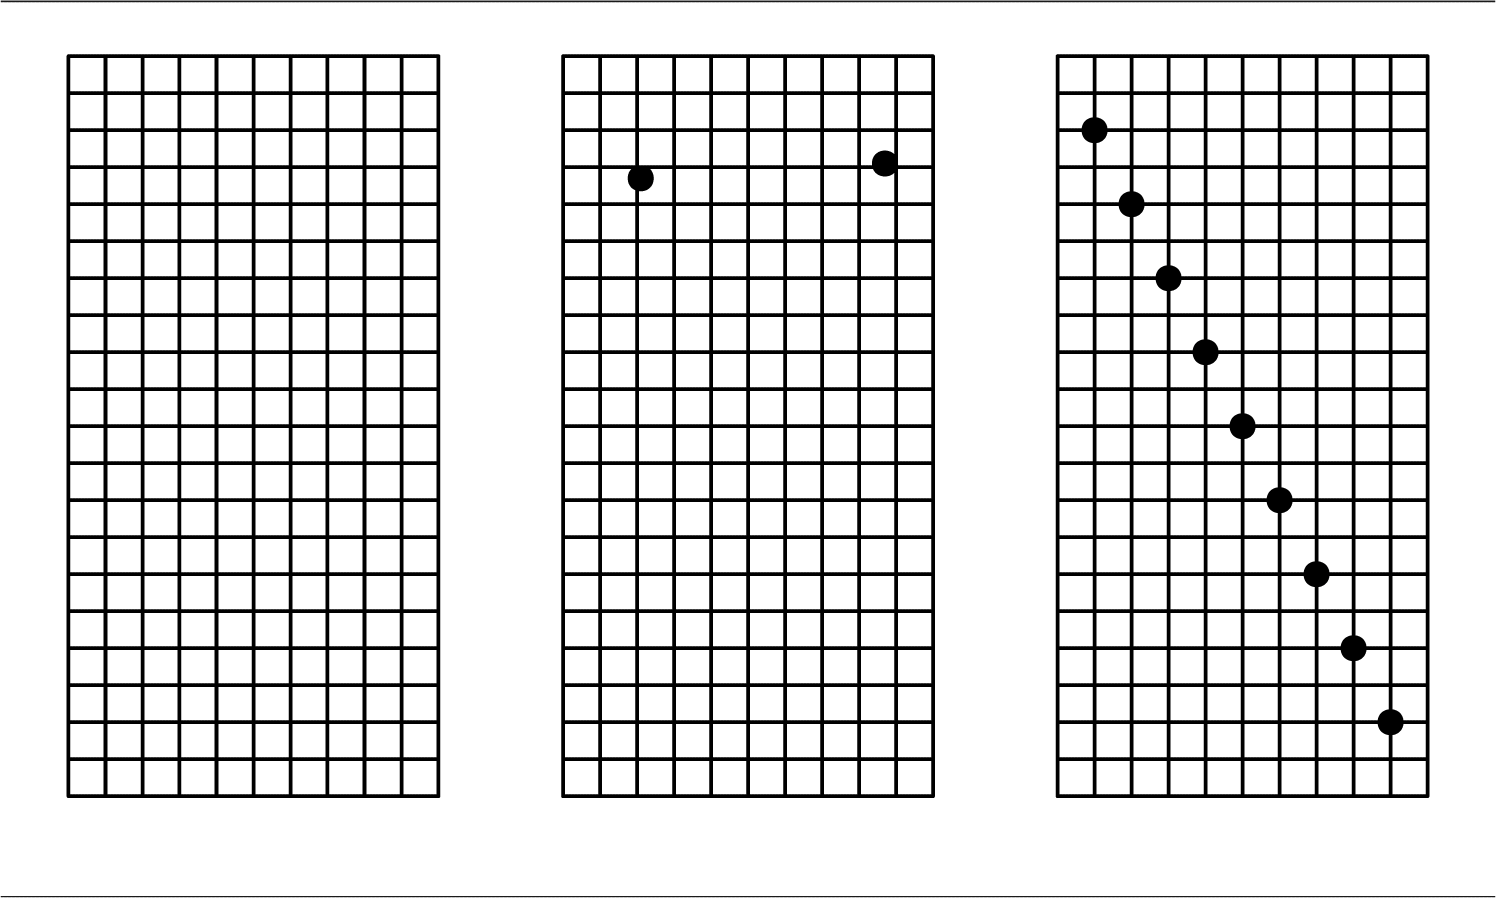
\includegraphics[width=0.85\textwidth]{images/00200.png}
  \caption{水球随机袭击模拟输出}
  \label{fig:random_attacks}
\end{figure}

\section{俄罗斯套娃}
\label{sec:ch09_russian_dolls}

维基百科将俄罗斯套娃（Russian doll）定义为“一组大小递减、层层嵌套的木制人偶”。每一层套娃都包裹着下一层更小的套娃，直到最里面是一个实心的、不再包含其他人偶的最内层人偶。

我们关注套娃的颜色属性，并用字符串来表示颜色。因此，除最内层外，每一层套娃都包含两项属性：自身的颜色、以及其内部包裹的套娃。我们用结构体来表示这种嵌套关系：
\begin{lstlisting}[language=BSL]
(define-struct layer [color doll])

; An RD（Russian doll，俄罗斯套娃）是以下之一：
; -- String
; -- (make-layer String RD)
; 解释：String 表示最内部的实心套娃的颜色；
;       (make-layer c d) 表示颜色为 c 且内部包含套娃 d 的套娃层。
\end{lstlisting}

例如，一个由黄色外层包裹着绿色中层、绿色中层包裹着红色最内层的三层套娃表示为：
\begin{lstlisting}[language=BSL]
(make-layer "yellow" (make-layer "green" "red"))
\end{lstlisting}

接下来设计函数 \code{depth} 计算套娃的总层数：
\begin{lstlisting}[language=BSL]
; RD -> Number
; 计算 an-rd 中共有多少个套娃
(check-expect (depth "red") 1)
(check-expect (depth (make-layer "yellow" (make-layer "green" "red"))) 3)

(define (depth an-rd)
  (cond
    [(string? an-rd) 1]
    [else (+ (depth (layer-doll an-rd)) 1)]))
\end{lstlisting}

\begin{exercise}{提取套娃的所有颜色}{154}
设计函数 \code{colors}：接收一个 \code{RD}，返回由逗号和空格分隔的所有外层到内层颜色的长字符串。例如上述三层套娃应返回 \code{"yellow, green, red"}。
\end{exercise}

\begin{exercise}{获取最内层颜色 inner}{155}
设计函数 \code{inner}：接收一个 \code{RD}，返回其最内层实心套娃的颜色。
\end{exercise}

\section{列表与世界}
\label{sec:ch09_lists_and_world}

有了列表之后，我们能够设计出比以往复杂得多的交互式世界程序（World Programs）。例如，在类似太空侵略者的射击游戏中，玩家不再受限于只能发射一枚导弹，而是可以任意多次按下空格键发射连续不断的弹幕。

\begin{notebox}[应用例题：弹幕射击模拟]
设计一个世界程序模拟发射子弹。每当玩家按下空格键，程序就在画布底端生成一颗子弹。所有子弹以每时钟节拍（tick）向上移动 1 像素的速度垂直上升。
\end{notebox}

首先确定常量：
\begin{lstlisting}[language=BSL]
(define HEIGHT 80)
(define WIDTH 100)
(define XSHOTS (/ WIDTH 2))

(define BACKGROUND (empty-scene WIDTH HEIGHT))
(define SHOT (triangle 3 "solid" "red"))
\end{lstlisting}

因为发射的子弹数量是动态且不确定的，所以必须使用列表来表示世界状态：
\begin{lstlisting}[language=BSL]
; A ShotWorld 是 List-of-numbers。
; 解释：列表中的每个数字代表一颗存活子弹当前的 y 坐标。
\end{lstlisting}

我们需要三个核心函数：
\begin{enumerate}
  \item \code{to-image}：将当前所有子弹绘制到背景画布上；
  \item \code{tock}：在每个时钟节拍使所有子弹的 $y$ 坐标减少 1（向上移动）；
  \item \code{keyh}：当按下空格键时，向列表中添加一颗新子弹（$y = \text{HEIGHT}$）。
\end{enumerate}

图~\ref{fig:list_based_world_program} 给出了完整的程序实现。

\begin{figure}[htbp]
  \centering
  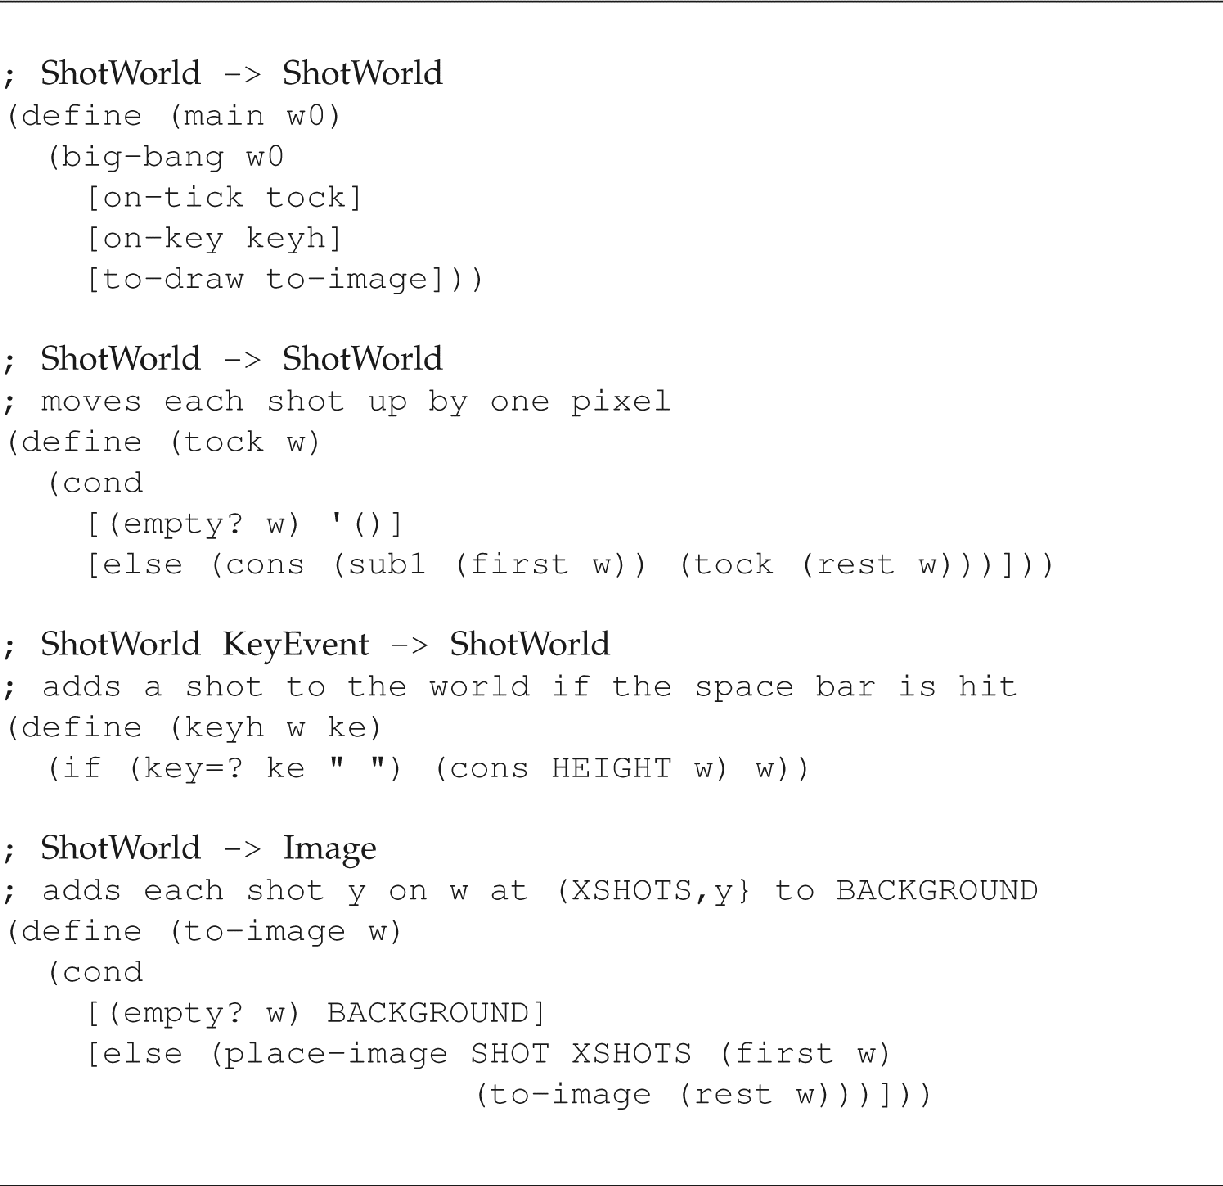
\includegraphics[width=0.9\textwidth]{images/00205.png}
  \caption{基于列表的世界程序完整代码}
  \label{fig:list_based_world_program}
\end{figure}

\begin{exercise}{运行弹幕程序}{156}
为图~\ref{fig:list_based_world_program} 中的程序编写完整的测试用例，并解释 \code{main} 函数的作用。随后在 DrRacket 中运行该程序。
\end{exercise}

\begin{exercise}{可配置常量测试}{157}
验证常量修改的灵活性：尝试修改画布高度为 220 像素、宽度为 30 像素、改变子弹颜色与发射位置等，观察程序是否只需修改单处常量即可正确响应。
\end{exercise}

\begin{exercise}{清除飞出屏幕的子弹}{158}
在图~\ref{fig:list_based_world_program} 中，飞出屏幕上边界的子弹虽然不再可见，但依然保留在列表数据中，导致列表越来越长。

设计改进版的 \code{tock} 函数：在使子弹向上移动的同时，自动剔除那些 $y < 0$ 的子弹。
\end{exercise}

\begin{exercise}{动态水球袭击世界程序}{159}
将练习 153 的方案转化为世界程序。主函数 \code{riot} 接收扔出的水球总数 $n$，以每秒 1 个的频率在随机位置投掷水球，并在窗口关闭时返回所有落点的 \code{Posn} 列表。
\end{exercise}

\section{关于列表与集合的旁注}
\label{sec:ch09_lists_and_sets}

读者可能会好奇：列表（List）与数学中的集合（Set）究竟有何异同？

从概念层面上看，集合主要用于程序设计前期的形式化讨论，而列表是编程语言中具体的一种数据结构。但更关键的区别在于处理数据时的核心关注点：
\begin{table}[htbp]
  \centering
  \caption{列表与集合的对比}
  \label{tab:lists_vs_sets}
  \begin{tabular}{lll}
    \hline
    \textbf{特征 (Property)} & \textbf{列表 (Lists)} & \textbf{集合 (Sets)} \\
    \hline
    元素归属 (Membership) & 众多特征之一 & 最核心的唯一判定标准 \\
    顺序 (Ordering) & 至关重要（有前后之分） & 无关紧要 \\
    出现次数 (\# of occurrences) & 有明确意义（允许重复） & 无关紧要（重复项不改变集合） \\
    规模大小 (Size) & 有限但可任意大 & 可以是有限的，也可以是无限的 \\
    \hline
  \end{tabular}
\end{table}

如果用有限列表来表示有限数字集合，可以采用两种策略（如图~\ref{fig:two_representations_of_sets} 所示）：
\begin{enumerate}
  \item \textbf{允许重复的列表}（\code{Son.L}）：直接使用列表，添加元素只需直接 \code{cons}，但删除元素时必须使用 \code{remove-all} 彻底清除所有重复项。
  \item \textbf{不允许重复的列表}（\code{Son.R}）：列表中的每个数字最多出现一次。添加元素时必须先检查是否已存在；而删除元素时只需使用普通的 \code{remove}。
\end{enumerate}

\begin{figure}[htbp]
  \centering
  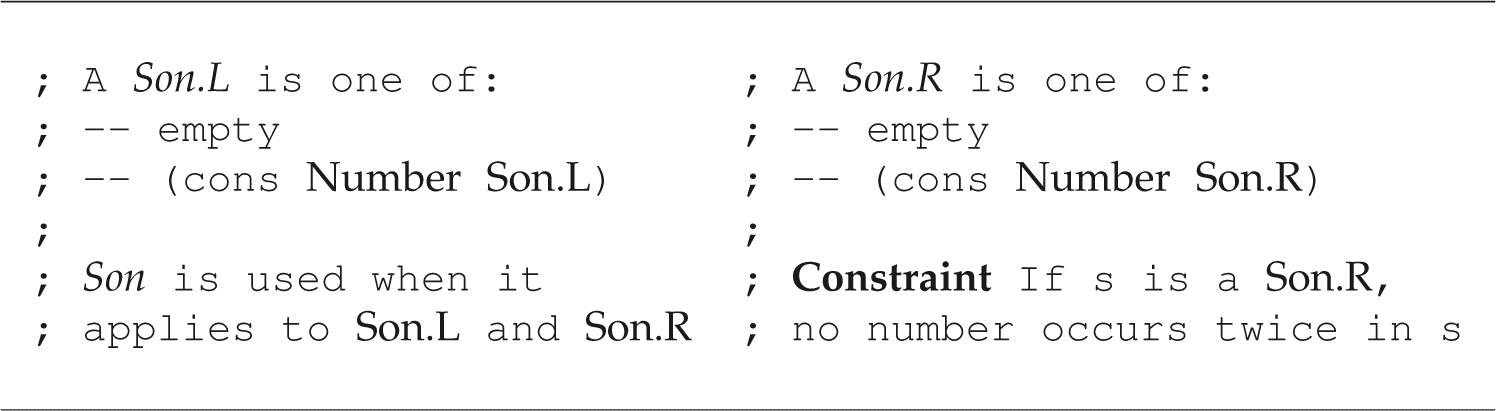
\includegraphics[width=0.85\textwidth]{images/00210.png}
  \caption{集合的两种列表数据表示形式}
  \label{fig:two_representations_of_sets}
\end{figure}

图~\ref{fig:set_functions_comparison} 对比了针对这两种集合表示形式的差集（删除元素）函数实现。

\begin{figure}[htbp]
  \centering
  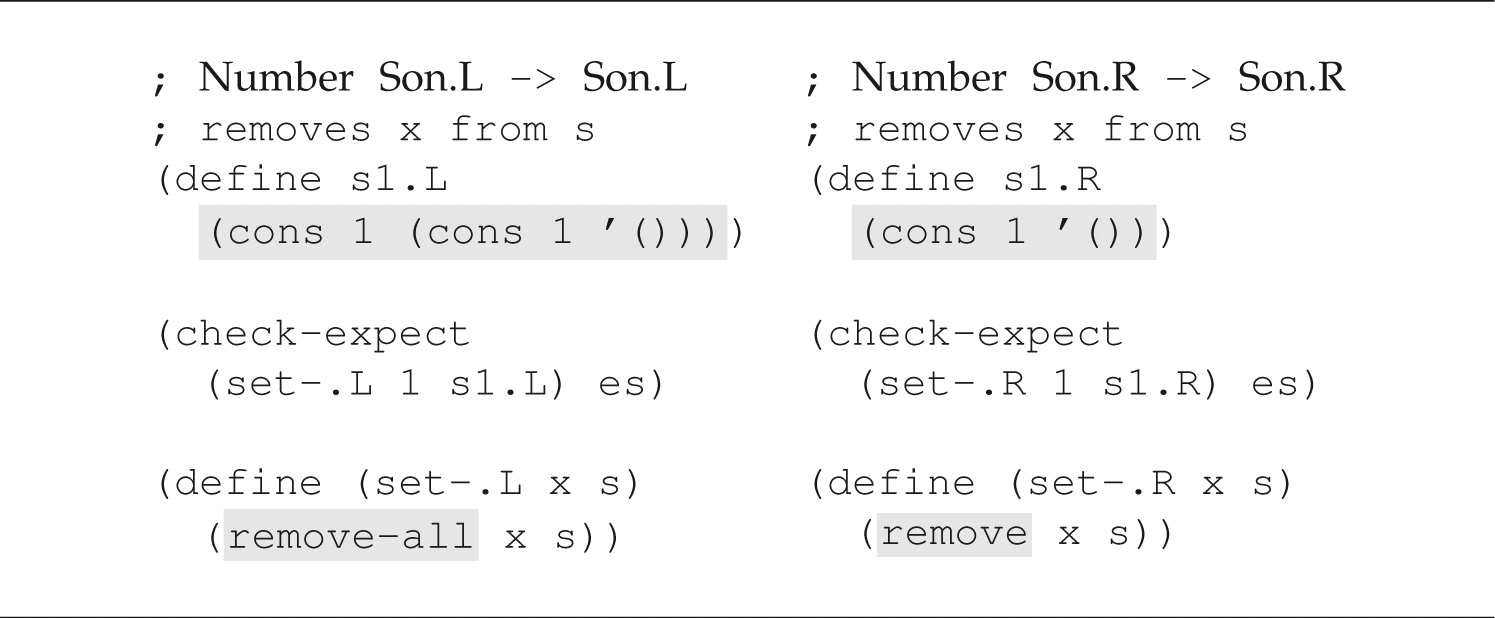
\includegraphics[width=0.85\textwidth]{images/00211.png}
  \caption{两种集合表示下的差集函数对比}
  \label{fig:set_functions_comparison}
\end{figure}

在测试集合函数时，由于集合元素的物理存储顺序并不重要，因此使用 BSL 提供的 \code{check-satisfied}（配合谓词如 \code{not-member-1?}）往往比硬编码特定列表顺序的 \code{check-expect} 更加稳健合理。

\begin{exercise}{集合添加元素函数 set+}{160}
分别针对 \code{Son.L}（允许重复）和 \code{Son.R}（不允许重复）设计添加元素函数 \code{set+.L} 与 \code{set+.R}。
\end{exercise}
